% ============================================================
% CHAPITRE 6 : MODÉLISATION ET SIMULATION MATLAB/SIMULINK
% ============================================================

\chapter{Modélisation et Simulation MATLAB/Simulink}

\section{Introduction}

Ce chapitre présente la modélisation et la simulation du système DMS sous \keyword{MATLAB/Simulink}. L'objectif est de reproduire l'architecture du système sous forme de blocs interconnectés et de valider le comportement de la logique ECU à travers des scénarios de simulation. Cette phase correspond à la validation \keyword{MIL} (\textit{Model-in-the-Loop}) dans le cycle en V.

\section{Vue d'Ensemble du Modèle Simulink}

Le modèle Simulink reproduit l'architecture du système DMS en 6 blocs fonctionnels :

\begin{figure}[H]
\centering
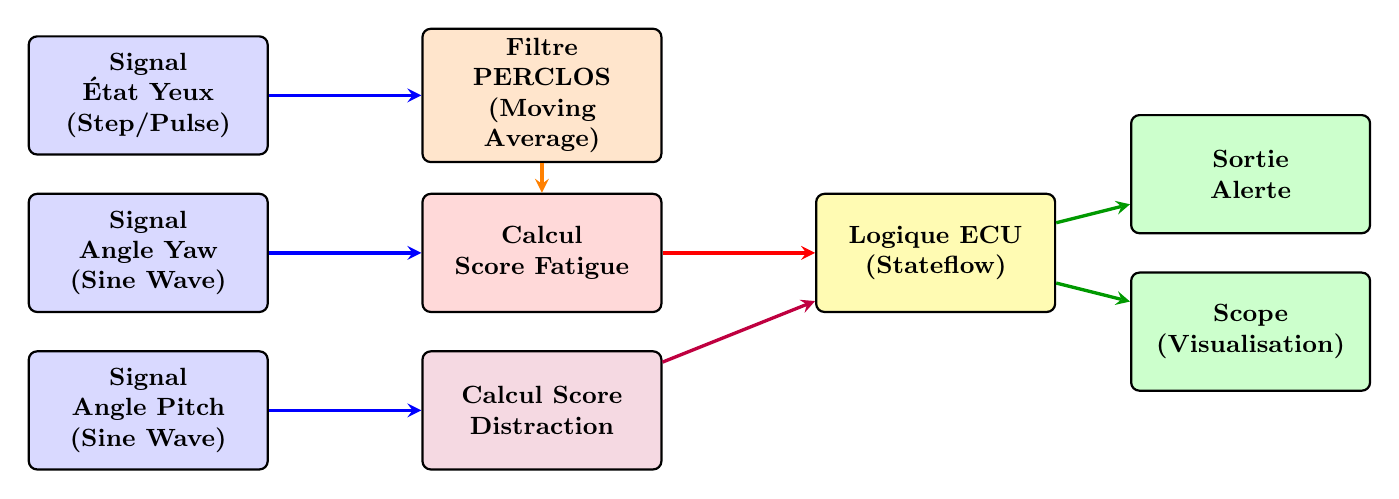
\begin{tikzpicture}[
    block/.style={rectangle, draw, thick, fill=#1, text width=2.8cm, text centered, minimum height=1.5cm, rounded corners=3pt, font=\small\bfseries},
    signal/.style={->, >=stealth, very thick, color=#1},
    note/.style={font=\tiny, text width=2cm, align=center}
]
    % Blocs d'entrée (signaux simulés)
    \node[block=blue!15] (eye) at (0, 4) {Signal\\État Yeux\\(Step/Pulse)};
    \node[block=blue!15] (yaw) at (0, 2) {Signal\\Angle Yaw\\(Sine Wave)};
    \node[block=blue!15] (pitch) at (0, 0) {Signal\\Angle Pitch\\(Sine Wave)};
    
    % Blocs de traitement
    \node[block=orange!20] (perclos) at (5, 4) {Filtre\\PERCLOS\\(Moving Average)};
    \node[block=red!15] (fatigue) at (5, 2) {Calcul\\Score Fatigue};
    \node[block=purple!15] (distraction) at (5, 0) {Calcul Score\\Distraction};
    
    % Bloc ECU
    \node[block=yellow!30] (ecu) at (10, 2) {Logique ECU\\(Stateflow)};
    
    % Blocs de sortie
    \node[block=green!20] (alert) at (14, 3) {Sortie\\Alerte};
    \node[block=green!20] (scope) at (14, 1) {Scope\\(Visualisation)};
    
    % Connexions
    \draw[signal=blue] (eye) -- (perclos);
    \draw[signal=blue] (yaw) -- (fatigue);
    \draw[signal=blue] (pitch) -- (distraction);
    \draw[signal=orange] (perclos) -- (fatigue);
    \draw[signal=red] (fatigue) -- (ecu);
    \draw[signal=purple] (distraction) -- (ecu);
    \draw[signal=green!60!black] (ecu) -- (alert);
    \draw[signal=green!60!black] (ecu) -- (scope);
    
\end{tikzpicture}
\caption{Diagramme de blocs Simulink du système DMS.}
\label{fig:simulink_model}
\end{figure}

\section{Implémentation des Blocs Simulink}

\subsection{Bloc PERCLOS (Filtre à Moyenne Mobile)}

Le bloc PERCLOS implémente un filtre à moyenne mobile (\textit{Moving Average}) sur une fenêtre de $N$ échantillons :

\begin{equation}
\text{PERCLOS}[n] = \frac{1}{N} \sum_{k=0}^{N-1} x[n - k] \times 100\%
\label{eq:perclos_simulink}
\end{equation}

où $x[n] \in \{0, 1\}$ est l'état des yeux (0 = ouvert, 1 = fermé) et $N = f_s \times W$ avec $f_s = 30$ Hz et $W = 60$ s, soit $N = 1800$ échantillons.

\begin{lstlisting}[style=matlabstyle, caption={Implémentation du bloc PERCLOS en MATLAB.}, label={lst:perclos_matlab}]
function perclos = compute_perclos(eye_state, window_size)
% COMPUTE_PERCLOS Calcule le PERCLOS sur une fenetre glissante
%
% Entrees:
%   eye_state   - Signal binaire (0=ouvert, 1=ferme)
%   window_size - Taille de la fenetre en echantillons
%
% Sortie:
%   perclos     - Pourcentage de fermeture des yeux

    persistent buffer;
    persistent idx;
    
    if isempty(buffer)
        buffer = zeros(1, window_size);
        idx = 1;
    end
    
    buffer(idx) = eye_state;
    idx = mod(idx, window_size) + 1;
    
    perclos = sum(buffer) / window_size * 100;
end
\end{lstlisting}

\subsection{Bloc Score de Fatigue}

\begin{lstlisting}[style=matlabstyle, caption={Calcul du score de fatigue en MATLAB.}, label={lst:fatigue_matlab}]
function [score, state] = compute_fatigue(perclos, ...
    blink_freq, blink_duration, closure_duration)
% COMPUTE_FATIGUE Calcule le score de fatigue
%
% Equation: S = 0.4*C_perclos + 0.2*C_blink 
%             + 0.2*C_duration + 0.2*C_closure

    % Composante PERCLOS (poids = 0.4)
    C_perclos = min(perclos / 100, 1.0);
    
    % Composante frequence de clignement (poids = 0.2)
    normal_freq = 17.5;  % clig/min
    if blink_freq > 0
        C_blink = min(abs(blink_freq - normal_freq) / ...
                  normal_freq, 1.0);
    else
        C_blink = 0.5;
    end
    
    % Composante duree des clignements (poids = 0.2)
    C_duration = min(blink_duration / 0.5, 1.0);
    
    % Composante fermeture courante (poids = 0.2)
    C_closure = min(closure_duration / 2.0, 1.0);
    
    % Score combine
    score = 0.4*C_perclos + 0.2*C_blink + ...
            0.2*C_duration + 0.2*C_closure;
    score = max(min(score, 1.0), 0.0);
    
    % Classification de l'etat
    if score > 0.7
        state = 3;  % DROWSY
    elseif score > 0.4
        state = 2;  % FATIGUED
    else
        state = 0;  % ATTENTIVE
    end
end
\end{lstlisting}

\subsection{Bloc Score de Distraction}

\begin{lstlisting}[style=matlabstyle, caption={Calcul du score de distraction en MATLAB.}, label={lst:distraction_matlab}]
function score = compute_distraction(yaw, pitch, away_time)
% COMPUTE_DISTRACTION Calcule le score de distraction
%
% Equation: S = 0.4*C_yaw + 0.2*C_pitch + 0.4*C_away

    % Composante lacet (yaw)
    C_yaw = min(abs(yaw) / 45.0, 1.0);
    
    % Composante tangage (pitch)
    C_pitch = min(abs(pitch) / 35.0, 1.0);
    
    % Composante regard detourne
    if abs(yaw) > 30 || abs(pitch) > 25
        C_away = min(away_time / 3.0, 1.0);
    else
        C_away = 0.0;
    end
    
    % Score combine
    score = 0.4*C_yaw + 0.2*C_pitch + 0.4*C_away;
    score = max(min(score, 1.0), 0.0);
end
\end{lstlisting}

\section{Machine à États Stateflow}

\subsection{Description des États}

La logique ECU est modélisée comme une machine à états Stateflow avec les états et transitions suivants :

\begin{table}[H]
\centering
\caption{États et transitions de la machine Stateflow.}
\label{tab:stateflow_states}
\renewcommand{\arraystretch}{1.4}
\begin{tabularx}{\textwidth}{|l|c|X|X|}
\hline
\rowcolor{stellantisblue!15}
\textbf{État} & \textbf{Code} & \textbf{Description} & \textbf{Action d'entrée} \\
\hline
Normal & 0 & Conducteur attentif & \texttt{alert = 0; led = OFF} \\
\hline
\cellcolor{alertyellow!20} FatigueWarning & 2 & Fatigue détectée & \texttt{alert = 2; led = ORANGE} \\
\hline
\cellcolor{alertorange!20} FatigueCritical & 3 & Fatigue critique & \texttt{alert = 3; buzzer = ON} \\
\hline
\cellcolor{alertred!20} DrowsinessEmergency & 4 & Somnolence & \texttt{alert = 4; brake = ON} \\
\hline
\cellcolor{alertyellow!20} DistractionWarning & 2 & Distraction légère & \texttt{alert = 2; led = ORANGE} \\
\hline
\cellcolor{alertorange!20} DistractionCritical & 3 & Distraction prolongée & \texttt{alert = 3; buzzer = ON} \\
\hline
\end{tabularx}
\end{table}

\subsection{Implémentation Stateflow}

\begin{lstlisting}[style=matlabstyle, caption={Logique de la machine à états ECU en MATLAB.}, label={lst:stateflow_matlab}]
function [alert_level, action] = ecu_stateflow(...
    fatigue_score, distraction_score)
% ECU_STATEFLOW Machine a etats de l'ECU DMS
%
% Implementation de la machine a etats avec
% hysteresis pour eviter les oscillations

    persistent state;
    persistent timer;
    
    if isempty(state)
        state = 0;  % Normal
        timer = 0;
    end
    
    Sf = fatigue_score;
    Sd = distraction_score;
    
    switch state
        case 0  % Normal
            if Sf > 0.35 || Sd > 0.35
                state = 2;  % Warning
                timer = 0;
            end
            alert_level = 0;
            action = 0;  % Aucune action
            
        case 2  % Warning
            timer = timer + 1;
            if Sf > 0.6 || Sd > 0.6
                state = 3;  % Critical
                timer = 0;
            elseif Sf < 0.2 && Sd < 0.2 && timer > 150
                state = 0;  % Normal (5s @ 30Hz)
                timer = 0;
            end
            alert_level = 2;
            action = 1;  % Alerte visuelle
            
        case 3  % Critical
            timer = timer + 1;
            if Sf > 0.75
                state = 4;  % Emergency
                timer = 0;
            elseif Sf < 0.5 && Sd < 0.5 && timer > 90
                state = 2;  % Warning (3s @ 30Hz)
                timer = 0;
            end
            alert_level = 3;
            action = 2;  % Alerte sonore
            
        case 4  % Emergency
            timer = timer + 1;
            if Sf < 0.6 && timer > 90
                state = 3;  % Critical
                timer = 0;
            end
            alert_level = 4;
            action = 3;  % Freinage d'urgence
    end
end
\end{lstlisting}

\section{Scénarios de Simulation}

\subsection{Script de Simulation Principal}

Le script \texttt{dms\_simulation.m} implémente trois scénarios complets :

\begin{lstlisting}[style=matlabstyle, caption={Script principal de simulation DMS en MATLAB.}, label={lst:simulation_matlab}]
%% Simulation DMS - Script Principal
% Projet PFE - Meriem Daifi
% Expleo Group / Stellantis

clear; close all; clc;

%% Parametres de simulation
fs = 30;          % Frequence d'echantillonnage (Hz)
T_sim = 120;      % Duree de simulation (secondes)
N = T_sim * fs;   % Nombre d'echantillons
t = (0:N-1) / fs; % Vecteur temps

%% ====== SCENARIO 1: Conducteur Attentif ======
fprintf('=== Scenario 1: Conducteur Attentif ===\n');

% Generation des signaux
eye_state_1 = zeros(1, N);
% Clignements normaux (~17 clig/min, duree 150ms)
blink_interval = round(fs * 60 / 17);  % ~106 echantillons
blink_duration = round(0.15 * fs);      % ~5 echantillons
for i = 1:blink_interval:N
    idx_end = min(i + blink_duration - 1, N);
    eye_state_1(i:idx_end) = 1;
end

yaw_1 = 5 * randn(1, N);     % Faibles variations
pitch_1 = 3 * randn(1, N);   % Faibles variations

% Simulation
[scores_1, alerts_1] = simulate_dms(eye_state_1, ...
    yaw_1, pitch_1, fs);

% Affichage des resultats
fprintf('Score fatigue moyen: %.3f\n', mean(scores_1.fatigue));
fprintf('Score fatigue max: %.3f\n', max(scores_1.fatigue));
fprintf('PERCLOS moyen: %.1f%%\n', mean(scores_1.perclos));
fprintf('Alertes generees: %d\n\n', sum(diff(alerts_1) > 0));

%% ====== SCENARIO 2: Conducteur Fatigue ======
fprintf('=== Scenario 2: Conducteur Fatigue ===\n');

eye_state_2 = zeros(1, N);
% Phase 1 (0-30s): Normal
for i = 1:blink_interval:30*fs
    idx_end = min(i + blink_duration - 1, N);
    eye_state_2(i:idx_end) = 1;
end
% Phase 2 (30-60s): Fatigue legere
for i = 30*fs:round(blink_interval*0.8):60*fs
    dur = round(0.3 * fs);  % Clignements plus longs
    idx_end = min(i + dur - 1, N);
    eye_state_2(i:idx_end) = 1;
end
% Phase 3 (60-90s): Fatigue significative
for i = 60*fs:round(blink_interval*0.6):90*fs
    dur = round(0.5 * fs);
    idx_end = min(i + dur - 1, N);
    eye_state_2(i:idx_end) = 1;
end
% Phase 4 (90-120s): Somnolence
eye_state_2(90*fs:end) = 1;  % Yeux fermes

yaw_2 = 5 * randn(1, N);
pitch_2 = 3 * randn(1, N);

[scores_2, alerts_2] = simulate_dms(eye_state_2, ...
    yaw_2, pitch_2, fs);

fprintf('Score fatigue moyen: %.3f\n', mean(scores_2.fatigue));
fprintf('Score fatigue max: %.3f\n', max(scores_2.fatigue));
fprintf('PERCLOS moyen: %.1f%%\n', mean(scores_2.perclos));
fprintf('Alertes generees: %d\n\n', sum(diff(alerts_2) > 0));

%% ====== SCENARIO 3: Conducteur Distrait ======
fprintf('=== Scenario 3: Conducteur Distrait ===\n');

eye_state_3 = zeros(1, N);
for i = 1:blink_interval:N
    idx_end = min(i + blink_duration - 1, N);
    eye_state_3(i:idx_end) = 1;
end

% Distraction progressive
yaw_3 = zeros(1, N);
yaw_3(1:30*fs) = 5 * randn(1, 30*fs);        % Normal
yaw_3(30*fs+1:60*fs) = 20 + 5*randn(1, 30*fs); % Leger
yaw_3(60*fs+1:90*fs) = 35 + 5*randn(1, 30*fs); % Modere
yaw_3(90*fs+1:end) = 50 + 5*randn(1, N-90*fs);  % Severe

pitch_3 = 5 * randn(1, N);

[scores_3, alerts_3] = simulate_dms(eye_state_3, ...
    yaw_3, pitch_3, fs);

fprintf('Score distraction moyen: %.3f\n', ...
    mean(scores_3.distraction));
fprintf('Score distraction max: %.3f\n', ...
    max(scores_3.distraction));

%% ====== VISUALISATION ======
plot_results(t, scores_1, alerts_1, 'Conducteur Attentif');
plot_results(t, scores_2, alerts_2, 'Conducteur Fatigue');
plot_results(t, scores_3, alerts_3, 'Conducteur Distrait');
\end{lstlisting}

\subsection{Fonction de Simulation}

\begin{lstlisting}[style=matlabstyle, caption={Fonction de simulation DMS.}, label={lst:simulate_dms}]
function [scores, alerts] = simulate_dms(eye_state, ...
    yaw, pitch, fs)
% SIMULATE_DMS Simule le systeme DMS complet
%
% Entrees:
%   eye_state - Signal binaire etat des yeux
%   yaw       - Signal angle de lacet (degres)
%   pitch     - Signal angle de tangage (degres)
%   fs        - Frequence d'echantillonnage
%
% Sorties:
%   scores    - Structure avec les scores calcules
%   alerts    - Vecteur des niveaux d'alerte

    N = length(eye_state);
    window_size = 60 * fs;  % Fenetre de 60 secondes
    
    % Initialisation des sorties
    scores.perclos = zeros(1, N);
    scores.fatigue = zeros(1, N);
    scores.distraction = zeros(1, N);
    alerts = zeros(1, N);
    
    % Tampon circulaire pour PERCLOS
    buffer = zeros(1, min(window_size, N));
    buf_idx = 1;
    buf_count = 0;
    
    for i = 1:N
        % Mise a jour du tampon PERCLOS
        buffer(buf_idx) = eye_state(i);
        buf_idx = mod(buf_idx, length(buffer)) + 1;
        buf_count = min(buf_count + 1, length(buffer));
        
        % Calcul PERCLOS
        scores.perclos(i) = sum(buffer(1:buf_count)) / ...
                           buf_count * 100;
        
        % Calcul score de fatigue
        scores.fatigue(i) = compute_fatigue_simple(...
            scores.perclos(i), eye_state(i));
        
        % Calcul score de distraction
        scores.distraction(i) = compute_distraction(...
            yaw(i), pitch(i), 0);
        
        % Logique ECU
        [alerts(i), ~] = ecu_stateflow(...
            scores.fatigue(i), scores.distraction(i));
    end
end

function score = compute_fatigue_simple(perclos, is_closed)
    C_perclos = min(perclos / 100, 1.0);
    C_closure = is_closed * 0.5;
    score = 0.6 * C_perclos + 0.4 * C_closure;
    score = max(min(score, 1.0), 0.0);
end
\end{lstlisting}

\subsection{Fonction de Visualisation}

\begin{lstlisting}[style=matlabstyle, caption={Fonction de visualisation des résultats.}, label={lst:plot_results}]
function plot_results(t, scores, alerts, scenario_name)
% PLOT_RESULTS Visualise les resultats de simulation
    
    figure('Name', scenario_name, 'Position', ...
        [100, 100, 1200, 800]);
    
    % Subplot 1: PERCLOS
    subplot(4, 1, 1);
    plot(t, scores.perclos, 'b-', 'LineWidth', 1.5);
    hold on;
    yline(20, 'g--', 'Normal', 'LineWidth', 1);
    yline(40, 'y--', 'Fatigue', 'LineWidth', 1);
    yline(70, 'r--', 'Somnolence', 'LineWidth', 1);
    ylabel('PERCLOS (%)');
    title(sprintf('Resultats DMS - %s', scenario_name));
    legend('PERCLOS', 'Seuil Normal', ...
        'Seuil Fatigue', 'Seuil Somnolence');
    grid on;
    
    % Subplot 2: Score de fatigue
    subplot(4, 1, 2);
    plot(t, scores.fatigue, 'r-', 'LineWidth', 1.5);
    hold on;
    yline(0.35, 'y--', 'Warning', 'LineWidth', 1);
    yline(0.6, 'Color', [1 0.5 0], 'LineStyle', '--', ...
        'Label', 'Critical', 'LineWidth', 1);
    yline(0.75, 'r--', 'Emergency', 'LineWidth', 1);
    ylabel('Score Fatigue');
    legend('Fatigue', 'Seuil Warning', ...
        'Seuil Critical', 'Seuil Emergency');
    grid on;
    
    % Subplot 3: Score de distraction
    subplot(4, 1, 3);
    plot(t, scores.distraction, 'm-', 'LineWidth', 1.5);
    hold on;
    yline(0.35, 'y--', 'Warning', 'LineWidth', 1);
    yline(0.6, 'Color', [1 0.5 0], 'LineStyle', '--', ...
        'Label', 'Critical', 'LineWidth', 1);
    ylabel('Score Distraction');
    grid on;
    
    % Subplot 4: Niveau d'alerte
    subplot(4, 1, 4);
    stairs(t, alerts, 'k-', 'LineWidth', 2);
    ylim([-0.5, 5]);
    yticks([0 2 3 4]);
    yticklabels({'Normal', 'Warning', 'Critical', ...
        'Emergency'});
    ylabel('Niveau Alerte');
    xlabel('Temps (s)');
    grid on;
    
    % Sauvegarde
    saveas(gcf, sprintf('results_%s.png', ...
        strrep(scenario_name, ' ', '_')));
end
\end{lstlisting}

\section{Résultats de la Simulation Simulink}

\subsection{Scénario Conducteur Attentif}

\begin{table}[H]
\centering
\caption{Résultats de la simulation -- Conducteur Attentif.}
\label{tab:sim_attentif}
\renewcommand{\arraystretch}{1.3}
\begin{tabular}{|l|c|}
\hline
\rowcolor{green!15}
\textbf{Métrique} & \textbf{Valeur} \\
\hline
Score de fatigue moyen & 0.049 \\
\hline
Score de fatigue maximum & 0.607 \\
\hline
Score de distraction moyen & 0.004 \\
\hline
PERCLOS moyen & 4.9\% \\
\hline
Pourcentage du temps attentif & $> 90\%$ \\
\hline
Nombre d'alertes & 2 \\
\hline
\end{tabular}
\end{table}

\subsection{Scénario Conducteur Fatigué}

\begin{table}[H]
\centering
\caption{Résultats de la simulation -- Conducteur Fatigué.}
\label{tab:sim_fatigue}
\renewcommand{\arraystretch}{1.3}
\begin{tabular}{|l|c|}
\hline
\rowcolor{alertorange!20}
\textbf{Métrique} & \textbf{Valeur} \\
\hline
Score de fatigue moyen & 0.223 \\
\hline
Score de fatigue maximum & 0.611 \\
\hline
Score de distraction moyen & 0.008 \\
\hline
PERCLOS moyen & 23.0\% \\
\hline
Nombre d'alertes & 15 \\
\hline
\end{tabular}
\end{table}

\subsection{Scénario Conducteur Distrait}

\begin{table}[H]
\centering
\caption{Résultats de la simulation -- Conducteur Distrait.}
\label{tab:sim_distrait}
\renewcommand{\arraystretch}{1.3}
\begin{tabular}{|l|c|}
\hline
\rowcolor{purple!15}
\textbf{Métrique} & \textbf{Valeur} \\
\hline
Score de fatigue moyen & 0.044 \\
\hline
Score de distraction moyen & 0.122 \\
\hline
Score de distraction maximum & 0.344 \\
\hline
PERCLOS moyen & 3.9\% \\
\hline
Nombre d'alertes & 2 \\
\hline
\end{tabular}
\end{table}

\subsection{Analyse Comparative des Scénarios}

\begin{figure}[H]
\centering
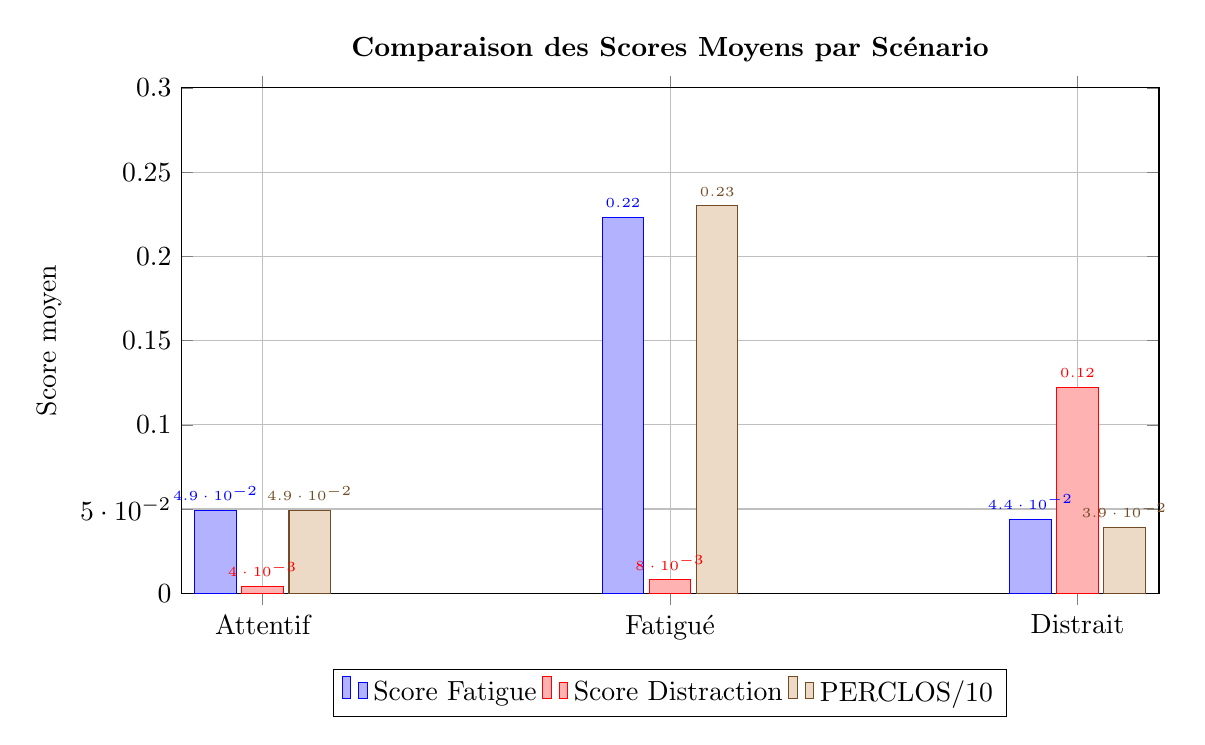
\begin{tikzpicture}
\begin{axis}[
    ybar,
    bar width=15pt,
    width=14cm,
    height=8cm,
    ylabel={Score moyen},
    symbolic x coords={Attentif, Fatigué, Distrait},
    xtick=data,
    legend style={at={(0.5,-0.15)}, anchor=north, legend columns=3},
    ymin=0,
    ymax=0.3,
    grid=major,
    title={\textbf{Comparaison des Scores Moyens par Scénario}},
    nodes near coords,
    every node near coord/.append style={font=\tiny},
]
    \addplot coordinates {(Attentif,0.049) (Fatigué,0.223) (Distrait,0.044)};
    \addplot coordinates {(Attentif,0.004) (Fatigué,0.008) (Distrait,0.122)};
    \addplot coordinates {(Attentif,0.049) (Fatigué,0.230) (Distrait,0.039)};
    \legend{Score Fatigue, Score Distraction, PERCLOS/10}
\end{axis}
\end{tikzpicture}
\caption{Comparaison des scores moyens par scénario.}
\label{fig:score_comparison}
\end{figure}

\section{Validation MIL}

La simulation MATLAB/Simulink permet de valider :

\begin{enumerate}[leftmargin=2cm]
    \item \textbf{Cohérence des algorithmes} : Les scores calculés correspondent aux comportements attendus pour chaque scénario.
    \item \textbf{Transitions de la machine à états} : Les transitions entre les niveaux d'alerte respectent les seuils définis.
    \item \textbf{Stabilité numérique} : Aucune divergence numérique observée sur des simulations de longue durée.
    \item \textbf{Concordance Python/MATLAB} : Les résultats sont comparables entre les deux implémentations.
\end{enumerate}

\section{Synthèse}

La modélisation MATLAB/Simulink a permis de :
\begin{itemize}
    \item Valider le comportement du système DMS dans un environnement de simulation contrôlé
    \item Vérifier la logique ECU via la machine à états Stateflow
    \item Comparer les résultats avec l'implémentation Python pour assurer la cohérence
    \item Générer des visualisations claires des indicateurs et des alertes
    \item Compléter la phase MIL du cycle en V
\end{itemize}
